\documentclass{beamer}
\usetheme{Copenhagen}
% \usepackage{metropolis_framesubtitle}
\usepackage[]{mathtools}
\definecolor{UBCblue}{rgb}{0.04706, 0.13725, 0.26667} % UBC Blue (primary)
\usecolortheme[named=UBCblue]{structure}
% \setbeamercolor{frametitle}{bg=black}
% \usefonttheme[]{serif}
% \usecolortheme{spruce}

\title[Lattices and Number Theory]{Can lattice points approximate irrationals?}
\subtitle[]{Exploring number theory through the regular system of points}
\author[Abhisruta Maity]{Abhisruta Maity}
\institute{21MS, IISER Kolkata}
\date{July 4, 2022}
\setbeamertemplate{title page}[default][colsep=-4bp,rounded=true]

\begin{document}
    \begin{frame}
        \titlepage
    \end{frame}

    \begin{frame}
        \frametitle{A look into lattice points}
        \framesubtitle{a.k.a. regular system of points in a plane}
        \begin{figure}
            \includegraphics[scale=0.40]{latt.png}
        \end{figure}

    \end{frame}
    \begin{frame}
        \frametitle{Generating lattice structure}
        \framesubtitle{Hero: Unit cells}
        \begin{columns}
            
            \column{0.5\textwidth}
                \begin{figure}
                    \centering
                    \includegraphics[scale=0.20]{unit.png}
                \end{figure}
            \column{0.5\textwidth}
                \begin{itemize}
                    \item<1-> A square can generate a square lattice. \pause
                    \item<2-> A parallelogram can generate a square lattice too. \pause
                \end{itemize}
                    
                    % These fundamental geometric objects which generate the lattice are called unit cells. 
    
                    % A lattice can be generated by square or parallelogram shaped unit cells having some specific shapes.
                    % Given any lattice structure, the unit cell corresponding to it is not unique.
                    \textbf{Given any lattice structure, the unit cell corresponding to it is not unique.}
        \end{columns}
    \end{frame}

    \begin{frame}
        \frametitle{Circle enters the room}
        \framesubtitle{Hunting lattice points inside a circle}
        \begin{figure}
            \includegraphics[scale=0.20]{scene1.png}
        \end{figure}
    \end{frame}

    \begin{frame}
        \frametitle{Circle entered the room}
        \framesubtitle{Approximating the area of the circle through lattice points}
        \begin{figure}
            \includegraphics[scale=0.20]{scene2.png}
        \end{figure}
    \end{frame}

    \begin{frame}
        \frametitle{Approximating the area}
        \framesubtitle{\(\pi\): I am coming!}
        \begin{figure}
            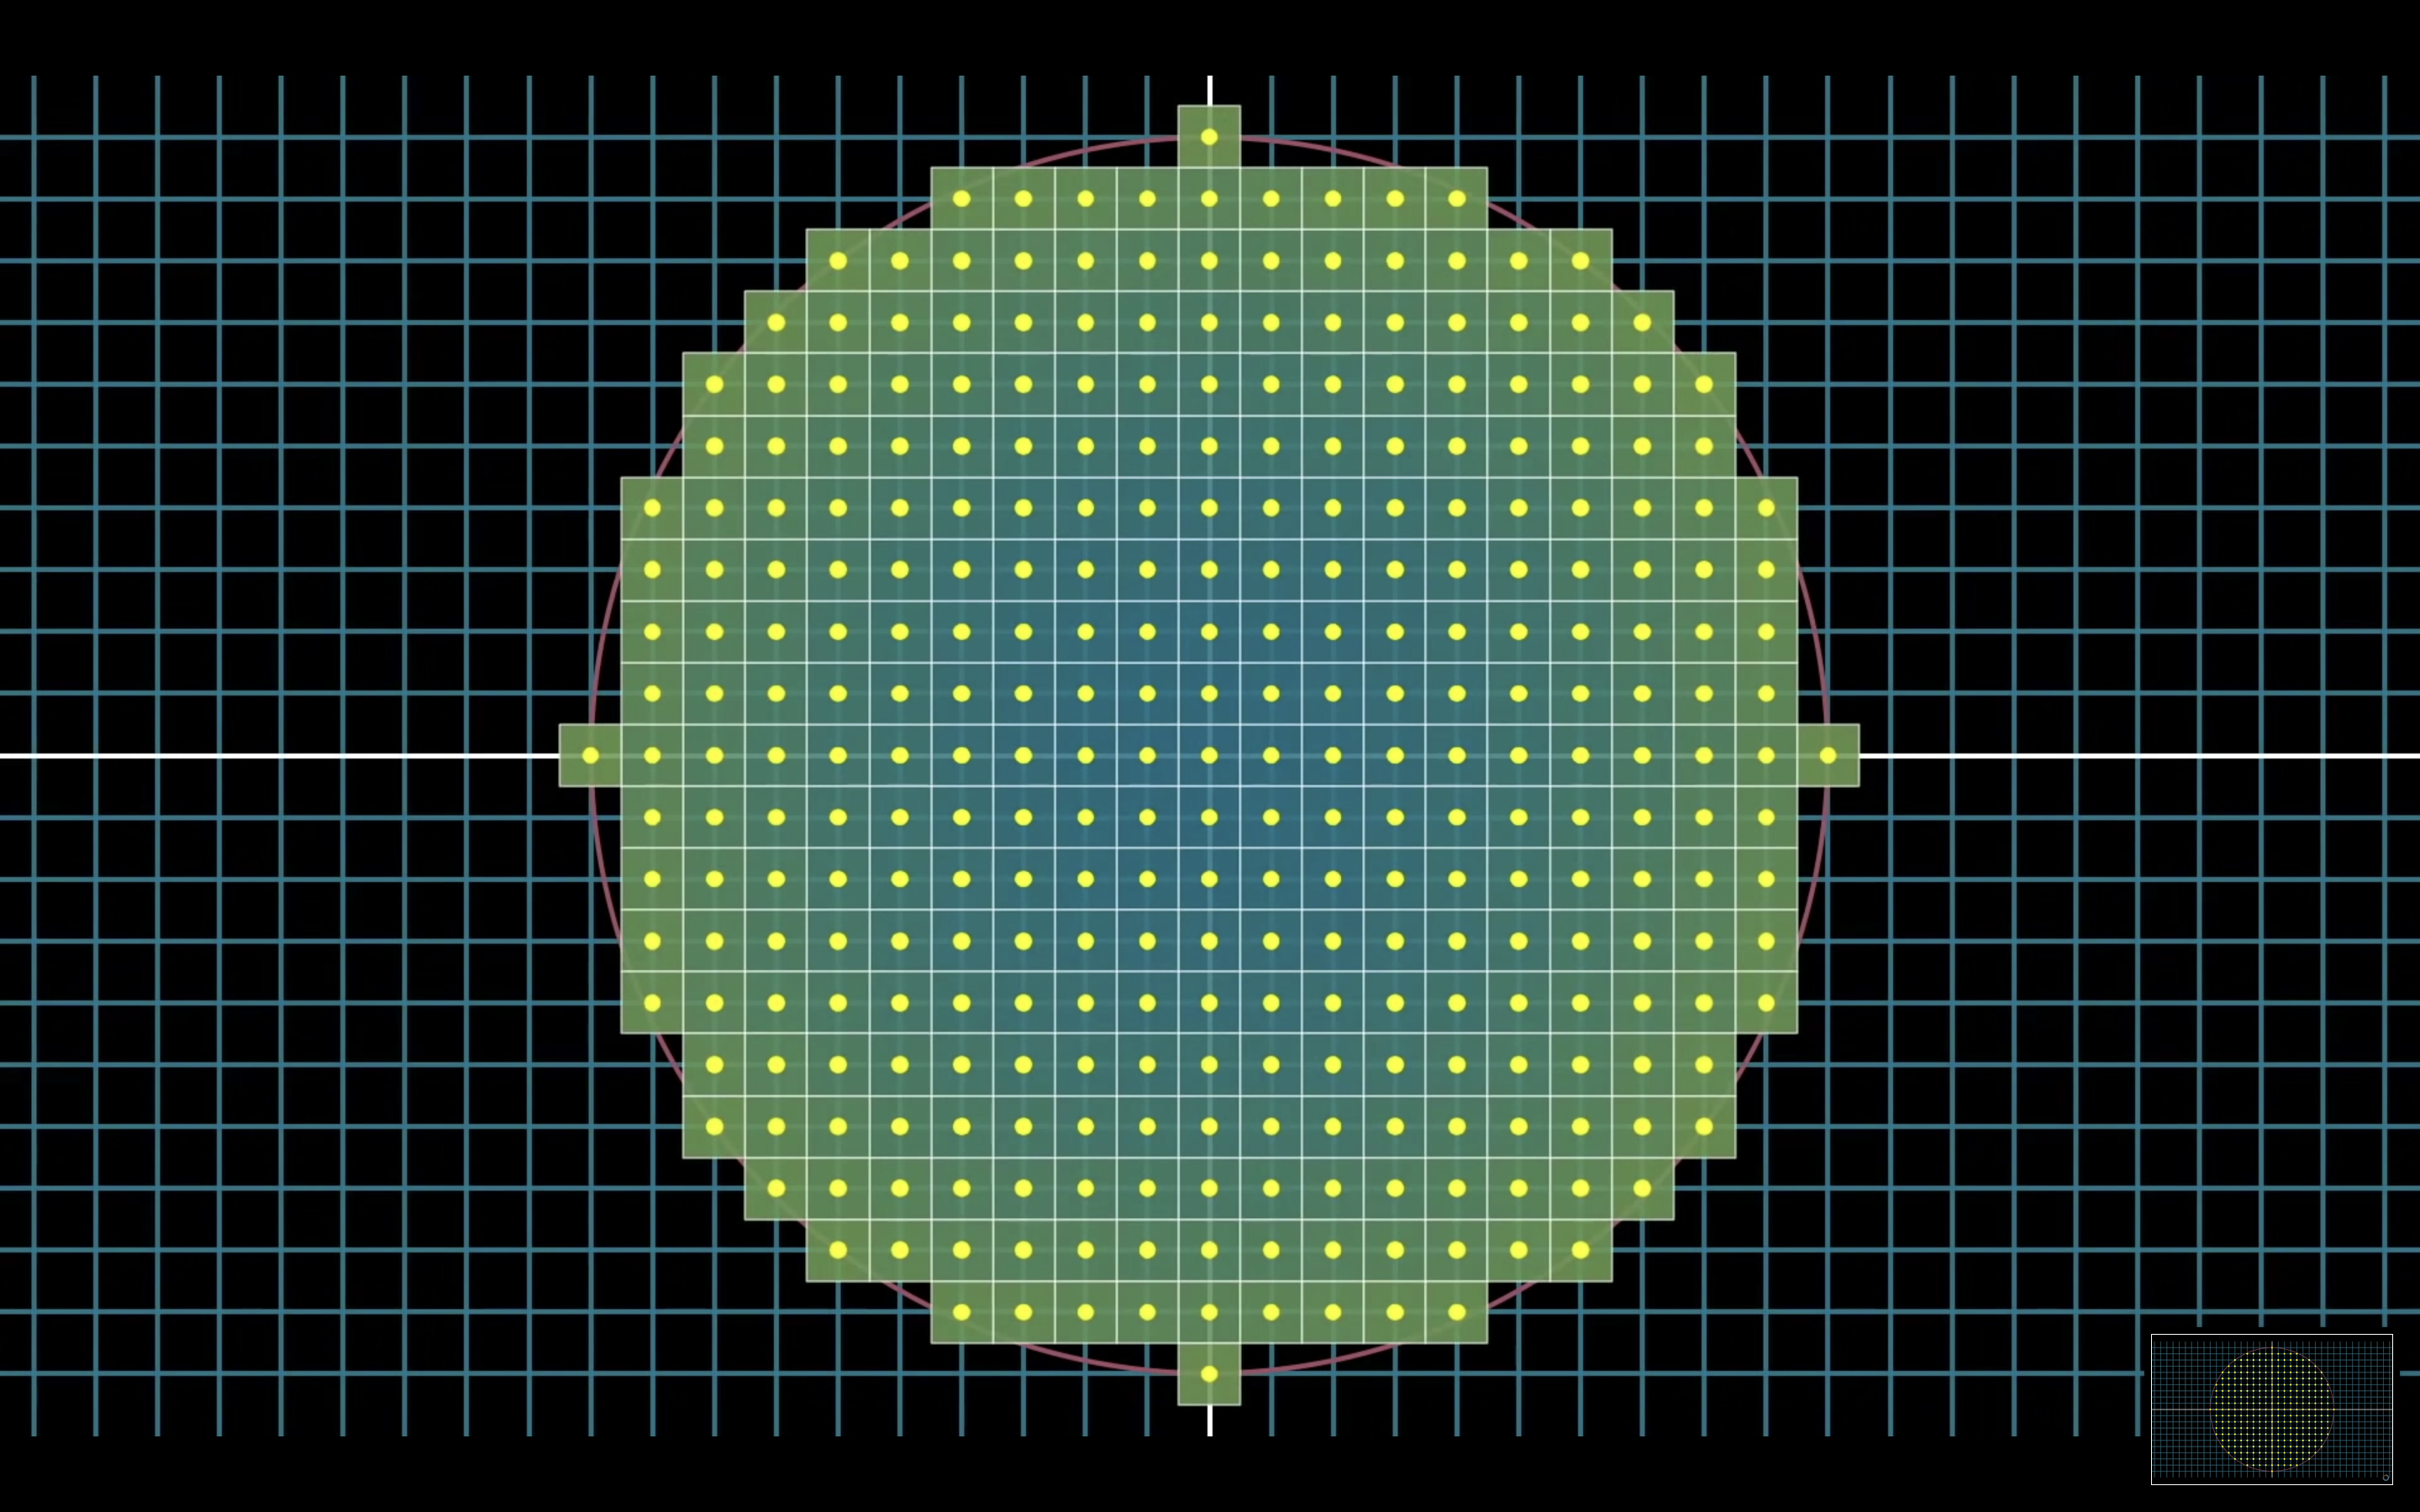
\includegraphics[scale=0.20]{scene3.png}
        \end{figure}
    \end{frame}

    \begin{frame}
        \frametitle{Is it a good approximation?}
        Suppose we assign the lattice points integer coordinates. Let the number of lattice points inside and on the circle is \(N(r)\) for a given integer radius \(r\). \pause We estimate \[|\pi r^2 - N(r)| < \varepsilon(r)\] \pause If \(\varepsilon(r)\) is \textbf{inversely correlated} with \(r\) then we are sure that this is indeed a good approximation. \\~\\ \pause

        This is the time we have to look back the previous diagram to estimate some bound on \(\varepsilon(r)\).
    \end{frame}

    \begin{frame}
        \frametitle{The bad squares}
        \framesubtitle{Can we estimate the area of the bad squares which is yielding the error?}
        \begin{figure}
            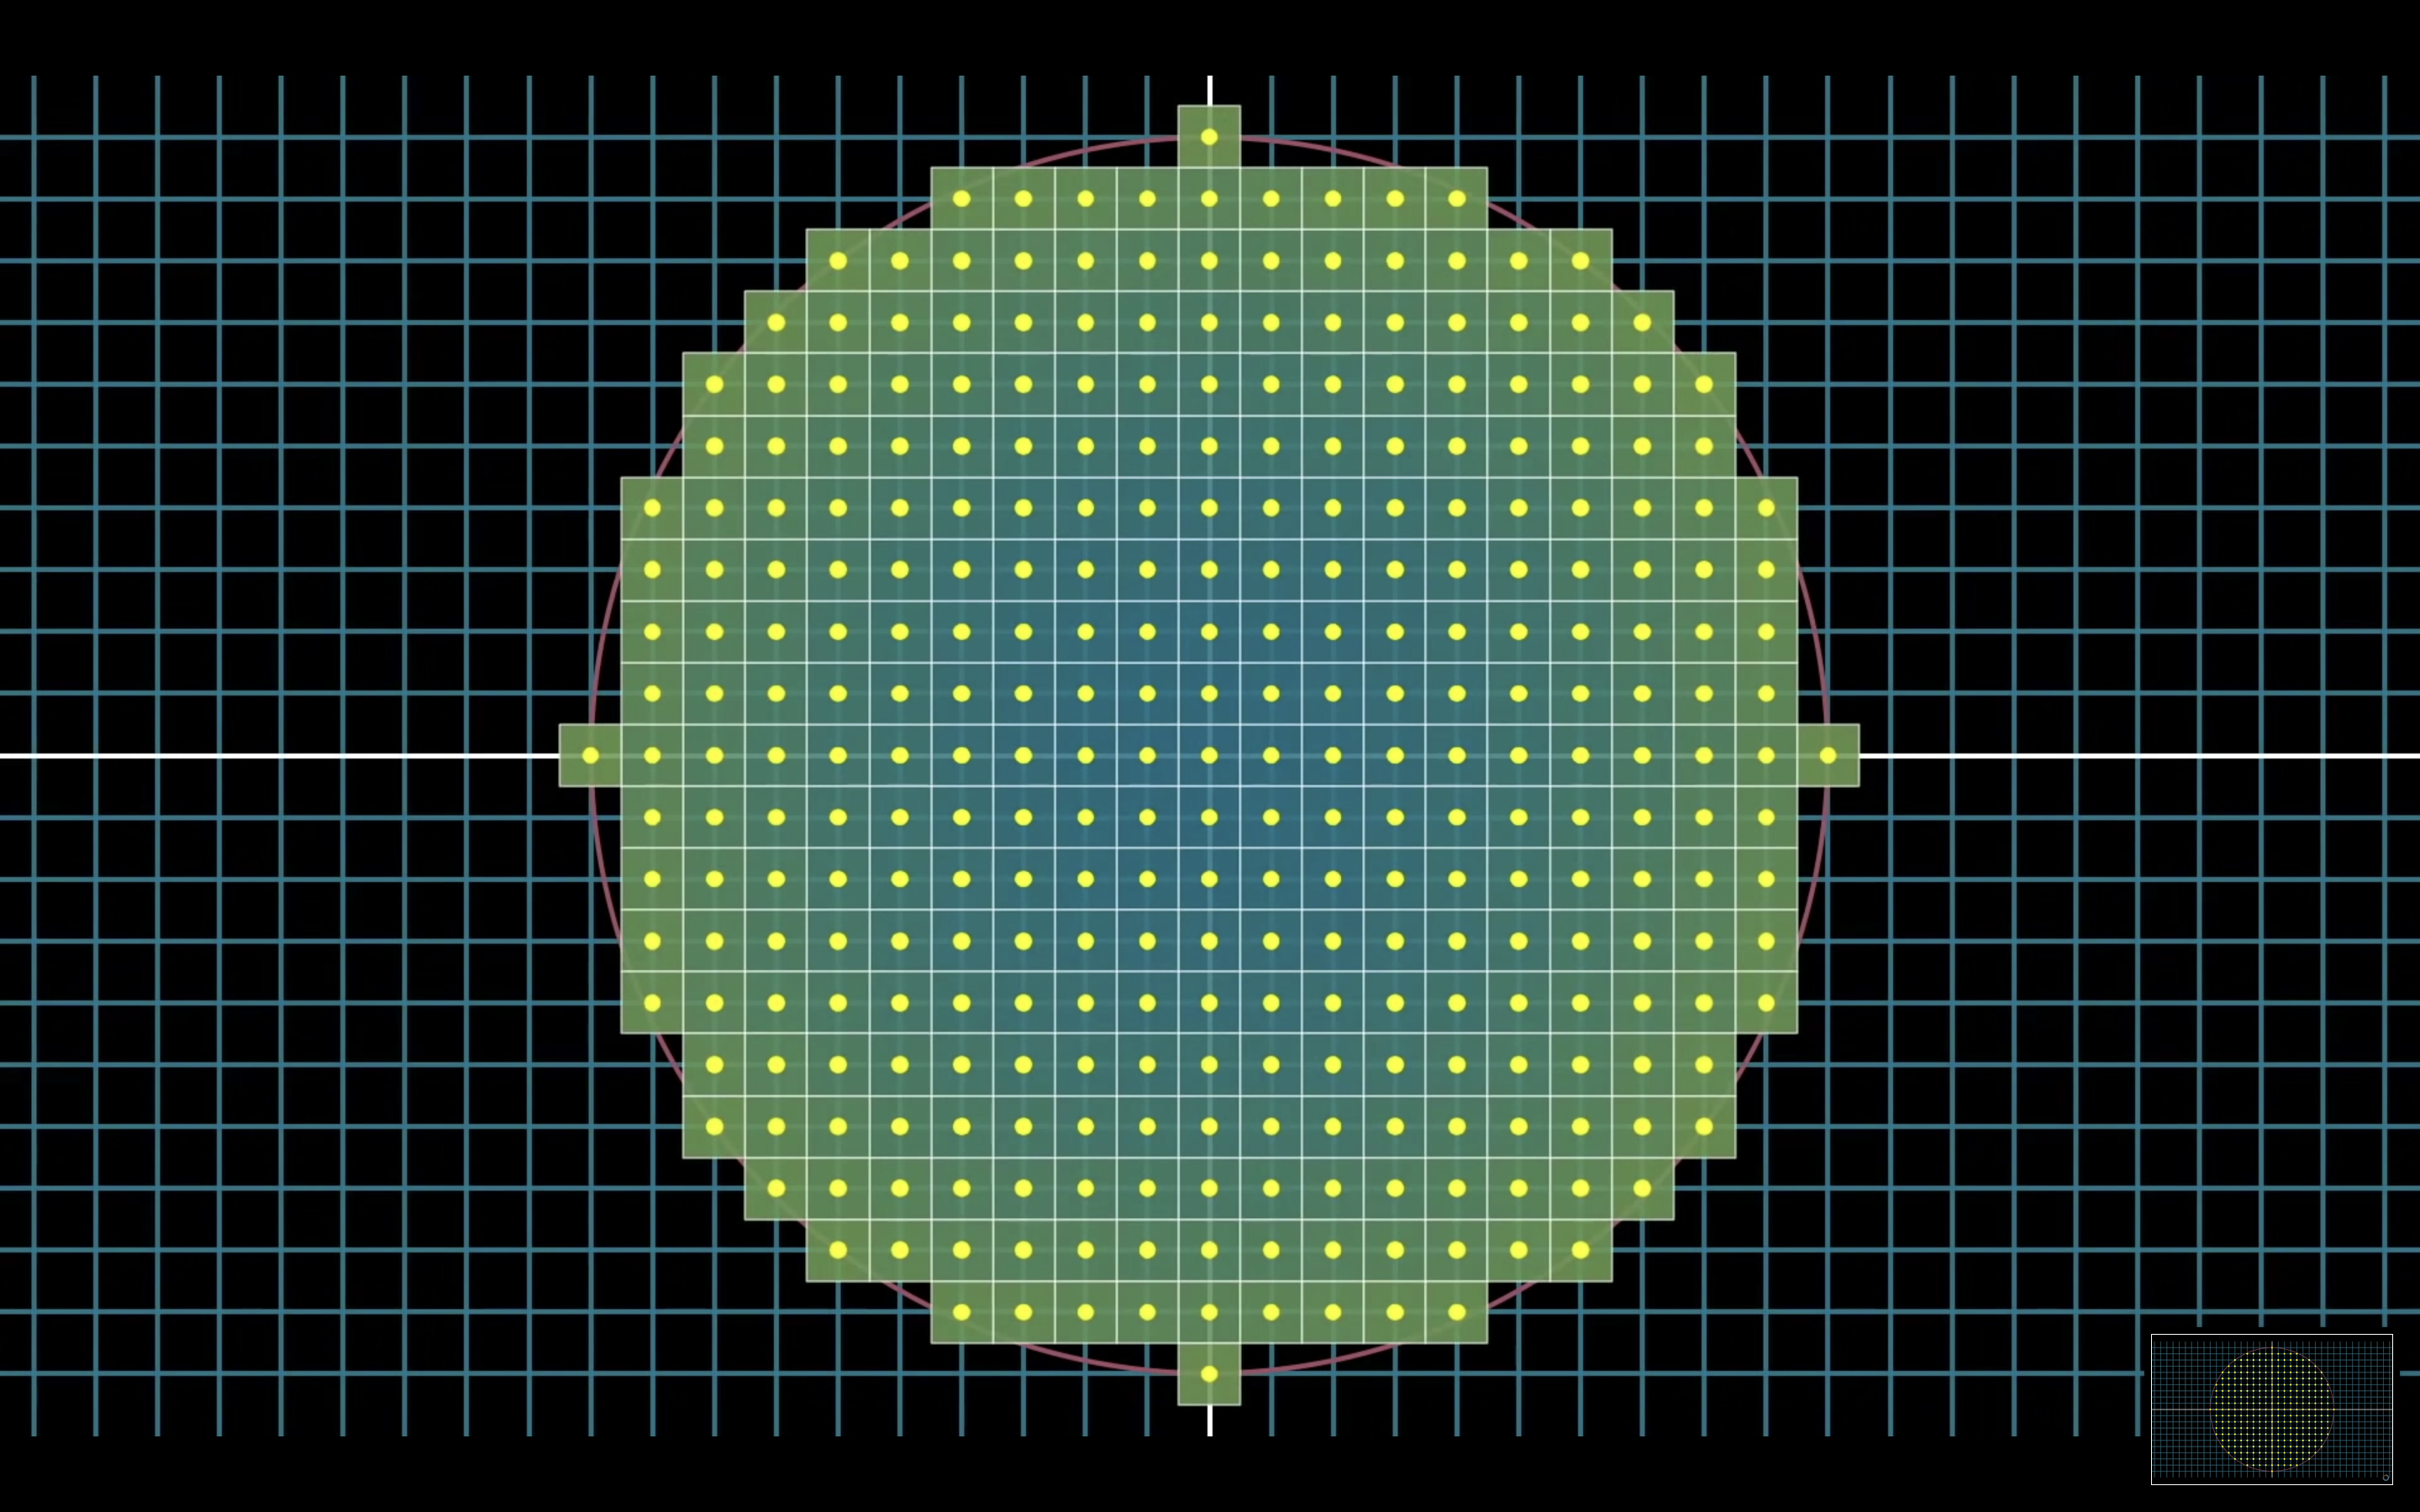
\includegraphics[scale=0.20]{scene3.png}
        \end{figure}
    \end{frame}

    \begin{frame}
        \frametitle{Estimating the bad area}
        The bad squares are entirely contained inside the annulus of smaller radius \(r - \sqrt{2}\) and bigger radius \(r + \sqrt{2}\). Hence the bad area \[\varepsilon(r) < E(r) = \pi [(r+\sqrt{2})^2 - (r-\sqrt{2})^2] = 4 \sqrt{2} \pi r\] Now it's moment to plug back!
    \end{frame}

    \begin{frame}
        \frametitle{Is it a good approximation?}
        Our previous estimation then becomes \[|\pi r^2 - N(r)| < \varepsilon(r) < 4 \sqrt{2} \pi r\] \pause Dividing by \(r^2\) yields \[\left|\pi - \frac{N(r)}{r^2}\right| < \frac{4 \sqrt{2} \pi}{r}\] \pause Look at the equation: \(N(r), r \in \mathbb{N}\). Hence, \(\frac{N(r)}{r^2}\) is a rational approximation of the irrational number \(\pi\) with the fact that we can approximate as close as we want, with increasing \(r\), subsequently decreasing the error term.
    \end{frame}

    \begin{frame}
        \frametitle{\(\sqrt{2}, e\) : What about approximating us?}

        Before diving into it, let's do some other works: deduce some important properties of the lattice structure. \\~\\ \pause

        Specifically, we will focus on \textbf{unit lattices}. Unit lattices are the lattice structures which are generated by the parallelograms or squares whose area is 1 unit\(^2\). 
    \end{frame}

    \begin{frame}
        \frametitle{Story of unit lattices}
        % Did you all remember the `solid state' chapter in +2 grade? We will talk about a concept we have learned in there, i.e., ``
        The distance of a lattice point to its first (nearest) neighbour (denote that distance as \(c\)). \pause \\~\\

        Suppose, you have a unit lattice structure.
        % Clearly, if we shear the unit cell parallelogram such that area remains 1 unit\(^2\), then \(c\) can be made arbitrarily small as a side of the parallelogram, forcing another side to be arbitrarily large \(\frac{1}{c}\). So, making \(c\) small is not that interesting.
        Lower bound of \(c\) is not interesting (in fact, it is 0). \pause \\~\\

        \begin{alertblock}{Question}
            Can we find some upper bound to it?
        \end{alertblock}
        
    \end{frame}

    \begin{frame}
        \frametitle{Finding max of the min distance}
        \begin{figure}
            \includegraphics[scale=0.45]{dist.png}
        \end{figure}
    \end{frame}

    % \begin{frame}
    %     \frametitle{Finding max of the min distance}
    %     In any given unit lattice, choose any pair of lattice points the distance between which is the minimum distance \(c\). On the straight lineg passing through these two points there must, according to the definition of the lattice, be infinitely many more lattice points spaced at intervals of length \(c\). The straight line \(h\) that is parallel tog and at a distance \(\frac{1}{c}\) from it must also contain infinitely many lattice points, but the strip betweeng and h cannot contain any. We now draw circles of radius \(c\) about all the lattice points on \(g\). The totality of circles covers a strip of the plane bounded by circular arcs. Every interior point of this strip is less than \(c\) distant from at least one lattice point and therefore, by the definition of \(c\), is not itself a lattice point. Hence \(\frac{1}{c}\) is greater than or equal to the shortest distance between the boundary of the strip and \(g\). Evidently this distance is the altitude of an equilateral triangle of side \(c\).
    % \end{frame}

    \begin{frame}
        \frametitle{Finding max of the min distance}
        Thus we have, \[\frac{1}{c} \geq \frac{c}{2}\sqrt{3}\] which yields an upper bound: \[\boxed{c \leq \sqrt{\frac{2}{\sqrt{3}}}}\]
        An easy exercise is to check when does the equality occur!
    \end{frame}

    \begin{frame}
        \frametitle{Approximation back again!}
        \begin{theorem}[Dirichlet's Approximation]
            For a given irrational \(\alpha\), the inequality, \[\left|\alpha - \frac{x}{y}\right| < \frac{1}{y^2}\] is satisfied by \textbf{infinitely many} integers \(x,y\).
        \end{theorem}
    \end{frame}

    \begin{frame}
        \frametitle{Approximation back again!}
        \framesubtitle{Focusing object: Quadratic forms}
        Consider the quadratic form of two variables \[Q(x,y) = ax^2 + 2hxy + by^2\] where \(a,h,b \in \mathbb{R}\). Inspecting \(Q(x,y)\), we get a representation of it in the following way: \pause \[Q(x,y) = \begin{bmatrix}
            x & y
        \end{bmatrix}
        \begin{bmatrix}
            a & h \\
            h & b
        \end{bmatrix}
        \begin{bmatrix}
            x \\
            y
        \end{bmatrix}\]
        The determinant of the matrix in between is called \emph{Discriminant} (denoted by \(D\)) of \(Q(x,y)\). For our problem, set \(D = 1\). Then \(a \neq 0\). WLOG, assume \(a > 0\).
    \end{frame}

    \begin{frame}
        \frametitle{Setting up a linear transformation}
        Notice that, now \(Q(x,y)\) can be written as \[Q(x,y) = \left(\sqrt{a}x + \frac{h}{\sqrt{a}}y\right)^2 + \left(\frac{1}{\sqrt{a}}y\right)^2\]
        Now set 
        \begin{align*}
            \tilde{x} &= \sqrt{a}x + \frac{h}{\sqrt{a}}y \\
            \tilde{y} &= \frac{1}{\sqrt{a}}y
        \end{align*}
        Note that, this is a linear transformation with determinant 1 (thus, area scaled is 1, i.e., the unit cell square is sheared into a parallelogram), pictorially shown in the next slide.
    \end{frame}

    \begin{frame}
        \frametitle{The shear}
        \begin{figure}
            \includegraphics[scale=0.29]{shear.png}
        \end{figure}
        Ignore the parameters in the diagrams.
    \end{frame}

    \begin{frame}
        \frametitle{The shear}
        If we allow \(x,y\) to run over integers (i.e., the pre-image lattice is ordinary unit square lattice), then the equation of the transformations represent set of points lying on the line \[\tilde{x} = h \tilde{y} + \sqrt{a}m\] and \[\tilde{y} = \frac{1}{\sqrt{a}}n\] where \(m, n \in \mathbb{Z}\). Which roughly looks like the dots in the above diagram. 
    \end{frame}
    \begin{frame}
        \frametitle{Key lemma}
        Consider, \[Q(x,y) = \tilde{x}^2 + \tilde{y}^2\] Thus \(\sqrt{Q(x,y)}\) represents the distance from the origin to the point \((\tilde{x},\tilde{y})\). The above ``first neighbour distance'' bound says that there will exist a point with the minimum distance \(c \leq \sqrt{\frac{2}{\sqrt{3}}}\).
    \end{frame}

    \begin{frame}

        \frametitle{Key lemma}

        Now, \[Q(x,y) = \tilde{x}^2 + \tilde{y}^2\] Thus \(\sqrt{Q(x,y)}\) represents the distance from the origin to the point \((\tilde{x},\tilde{y})\). The above ``first neighbour distance'' bound says that there will exist a point with the minimum distance \(c \leq \sqrt{\frac{2}{\sqrt{3}}}\). \\~\\
        
        \begin{lemma}
            Take integer lattice \(\mathbb{Z}^2\). After we transform it through a linear transformation as discussed above whose determinant is 1, then there exists \(x,y \in \mathbb{Z}\) such that \[Q(x,y) \leq \frac{2}{\sqrt{3}}\] where \((x,y) \mapsto (\tilde{x}, \tilde{y})\) and \(Q(x,y)= \tilde{x}^2 + \tilde{y}^2\).
        \end{lemma}
    \end{frame}

    \begin{frame}
        \frametitle{The final bash}

        Let \(\epsilon > 0\). Consider the quadratic form \[Q(x,y) = \left(\frac{\alpha y - x}{\epsilon}\right)^2 + \epsilon^2y^2\] whose determinant is \[\frac{1}{\epsilon^2}\left(\frac{\alpha^2}{\epsilon^2} + \epsilon^2\right) - \frac{\alpha^2}{\epsilon^4} = 1\] \pause From the previous lemma, it follows that, \(\exists x,y \in \mathbb{Z}\) such that \[Q(x,y) = \left(\frac{\alpha y - x}{\epsilon}\right)^2 + \epsilon^2y^2 \leq \frac{2}{\sqrt{3}}\] \pause Consequently, as a \emph{fortiori} we have two simultaneous inequalities (projection of radius is lesser than or equal to the radius!): \[\left|\frac{\alpha y - x}{\epsilon}\right| \leq \sqrt{\frac{2}{\sqrt{3}}}, \quad |\epsilon y| \leq \sqrt{\frac{2}{\sqrt{3}}}\]
    \end{frame}

    \begin{frame}
        \frametitle{The final bash}
        Assume \(y \neq 0\). Rearranging the inequalities a bit and using the fact that \(|y| \geq 1\) and \(y \in \mathbb{Z}\backslash\{0\}\), we have \[\left|\alpha - \frac{x}{y}\right| \leq \frac{\epsilon}{|y|}\sqrt{\frac{2}{\sqrt{3}}} \leq \epsilon\sqrt{\frac{2}{\sqrt{3}}}, \quad |y| \leq \frac{1}{\epsilon}\sqrt{\frac{2}{\sqrt{3}}}\] \pause Suppose \(\alpha\) is irrational. Then LHS of the left inequalities must be positive. \pause
        \begin{itemize}
            \item<1-> Fix some \(\epsilon > 0\).
            \item<2-> By the argument we are guranteed to get integer solutions \(x,y\) which satisfies both the inequalities.
        \end{itemize}
        Then rational number \(\frac{x}{y}\) approximates the irrational \(\alpha\).
    \end{frame}
    \begin{frame}
    \frametitle{The refinement}
        Next step is to refine the approximation: 
        \begin{itemize}
            \item<1-> Reduce the \(\epsilon\) so that it becomes a smaller positive number than before. \pause
            \item<2-> Compute the integer solutions, say one of them in this case is \(x_0, y_0\). \pause
            \item<3-> From the first inequality, the bound of the error term of approximation reduces (due to reduction of \(\epsilon\)). \pause
        \end{itemize}
        \textbf{But the approximation may get worse!} \pause
        \begin{itemize}
            \item Take \(\epsilon < \frac{1}{2}\left|\alpha - \frac{x_0}{y_0}\right|\) \pause
            \item Again, the previous argument ensures the existence of new integer solutions \(x_1, y_1\), which indeed is better than \(x_0, y_0\).
        \end{itemize}
        This process can be continued indefinitely to get as much good accuracy as we want.
        
        % infinitely many pairs of \((x,y)\) setting \(\epsilon\) smaller and smaller, which forces the error in approximating \(\alpha\) by \(\frac{x}{y}\) \[\left|\alpha - \frac{x}{y}\right| \to 0\] Thus through this in the decreasing \(\epsilon\) process, we generate a sequence of \((x,y)\) which approximates irrational \(\alpha\), as precise as we desire. 
    \end{frame}

    \begin{frame}
        \frametitle{Arriving to the end of the story!}
        \framesubtitle{Or, it is the start?}
        % On other side of the process, we have the concise inequality \[\left|\alpha - \frac{x}{y}\right| \leq \frac{2}{\sqrt{3}} \frac{1}{y^2}\] which asserts 
        \begin{theorem}[Weaker form of Dirichlet's Approximation] 
            Suppose \(\alpha\) is an irrational number. \(\forall \epsilon > 0 \quad \exists x, y \in \mathbb{Z}\) such that the two simultaneous inequalities hold: \[\left|\alpha - \frac{x}{y}\right| \leq \frac{\epsilon}{|y|}\sqrt{\frac{2}{\sqrt{3}}}, \quad |y| \leq \frac{1}{\epsilon}\sqrt{\frac{2}{\sqrt{3}}}\] 
            By the above refinement process, we are guaranteed to generate an \textbf{infinite sequence} of \(x,y \in \mathbb{Z}\), such that \[\left|\alpha - \frac{x}{y}\right| \leq \frac{2}{\sqrt{3}} \frac{1}{y^2}\]
        \end{theorem}
        % that rather a good approximation can be obtained by the sequence of \((x,y)\) with comparatively small denomenators, since the error is inversely proportional to square of the denominator. 
        
        % \\~\\

        % This turns out to be a little bit weaker version of the \emph{Dirichlet's Approximation theorem}, where the error bound has only the inverse of square of the denominator.
    \end{frame}
    \begin{frame}
        \frametitle{Arriving to the end of the story!}
        \framesubtitle{Or, it is the start?}
        \begin{example}
            We want to approximate \(\sqrt{43}\). Take \(\epsilon = 0.5\), then \(\frac{x}{y} = \frac{6}{1}\) is the only solution satisfying both the inequalities. Reducing \(\epsilon\) a bit, say \(\epsilon = 0.2 < \frac{1}{2}\left|\sqrt{43} - \frac{6}{1}\right|\), we get two solutions \(\frac{x}{y}\) = \(\frac{13}{2}\) and \(\frac{33}{5}\), which are guaranteed to have higher accuracy of approximation than before.
        \end{example}
    \end{frame}
    
    \begin{frame}
        \begin{alertblock}{Remark}
            Not only the above, as we go along the sequence, \textbf{eventually} the approximation gets better as well as \textbf{quickly} since the error bound is proportional to the inverse of the square of the denominator, than randomly setting a denominator and then finding a multiple of that which ``fits" with the irrational number.
        \end{alertblock}
    \end{frame}
    \begin{frame}
        \frametitle{Thank You! Identity.}
        \textbf{References and Acknowledgements: }
        \begin{enumerate}
            \item David Hilbert, S. Cohn-Vossen. \emph{Geometry and the Imagination}. American Mathematical Society, RH. 1952.
            \item Paul Erdős, János Surányi. \emph{Topics in the Theory of Numbers}. Springer. 2003.
            \item 3Blue1Brown YouTube channel.
            \item Google images library.
        \end{enumerate}
    \end{frame}
    % \begin{frame}
    %     \frametitle{Computation aspect}
    %         With this way we will always be able to get ``good'' approximation with as much accuracy as we want, than randomly setting a denominator and then finding a multiple of that which ``fits" with the irrational number.
    % \end{frame}
\end{document}

% verbally summarise before starting.

% lattice points why they are useful in approximating irrational numbers. present different ways to